\begin{problem}{The Great Box Shuffle}{standard input}{standard output}{1 second}{256 megabytes}

In the heart of Algoria, during the annual festival, a thrilling challenge called \textbf{The Great Box Shuffle} captivates all who attend. The challenge involves two long rows of enchanted boxes, each containing a collection of mystical items. The boxes in the two rows are enchanted in such a way that, with a bit of magic, their contents can be shuffled to match each other.

\begin{center}
  \def \htmlPixelsInCm {45}  % pixels in 1 centimeter in HTML mode
  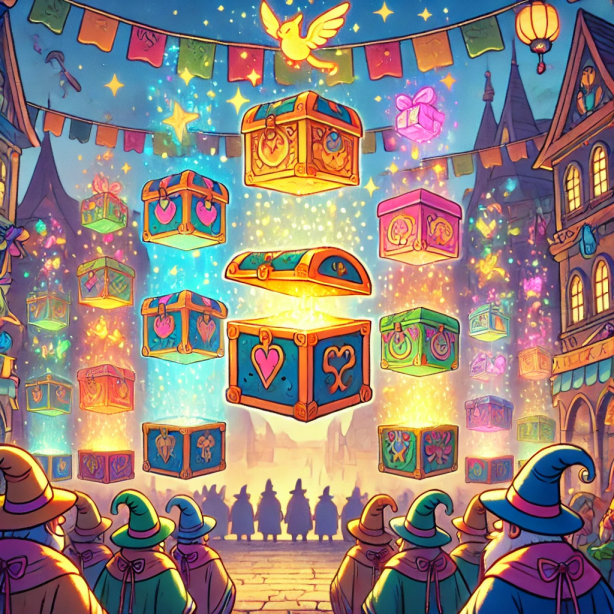
\includegraphics[width=4cm]{box.png} \\
  \small{The Great Box Shuffle festival in Algoria}
\end{center}

You are the chosen contestant this year, and your task is to determine if specific groups of boxes from the first row can be rearranged to perfectly match groups of boxes from the second row. However, the magical rules of the festival only allow you to shuffle the items within a contiguous group of boxes, rotating them either to the left or right.

Throughout the challenge, you will be given several queries. Each query will ask if a particular group of boxes from the first row can be rearranged to match a group of boxes from the second row using the allowed shuffling magic.

More formally, you are given two sequences \( A \) and \( B \), each of length \( N \). You need to answer \( q \) queries. Each query is defined by four integers \( l_1 \), \( r_1 \), \( l_2 \), and \( r_2 \). For each query, you must determine if the subarray \( A[l_1..r_1] \) can be shuffled to match the subarray \( B[l_2..r_2] \) by rotating the items within the selected segment.

\InputFile
\begin{itemize}
    \item The first line contains a single integer \( N \) --- the number of boxes in each row.
    \item The second line contains \( N \) integers \( A_1, A_2, \dots, A_N \), where \( A_i \) represents the number of items in the \( i \)-th box of the first row.
    \item The third line contains \( N \) integers \( B_1, B_2, \dots, B_N \), where \( B_i \) represents the number of items in the \( i \)-th box of the second row.
    \item The fourth line contains a single integer \( q \) --- the number of queries.
    \item The next \( q \) lines each contain four integers \( l_1 \), \( r_1 \), \( l_2 \), and \( r_2 \). For each query, you need to determine whether it is possible to shuffle the group of boxes from the first row (from box \( l_1 \) to box \( r_1 \)) to match the corresponding group of boxes from the second row (from box \( l_2 \) to box \( r_2 \)).
\end{itemize}

\section*{Constraints}

\begin{itemize}
    \item \( 1 \leq N, Q \leq 200,000 \)
    \item \( 1 \leq l_1 \leq r_1 \leq N \)
    \item \( 1 \leq l_2 \leq r_2 \leq N \)
    \item \( 1 \leq A_i, B_i \leq N \)
\end{itemize}

\OutputFile
For each query, print \texttt{Yes} if you can shuffle the group of boxes from the first row to match the corresponding group from the second row. Otherwise, print \texttt{No}.

\Scoring
There are some subtasks in this problem, you will get the percentage of score if you pass the subtask

\begin{center}
  \begin{tabular}{ | c | c | c | c | } \hline
    \bf{Subtask} &
    \bf{Condition} &
    \bf{Score} &
    \bf{Additional Limitations} \\ \hline
    $1$ & $n,q \le 1000$ & $40\%$ & None \\ \hline
    $2$ & No additional constraints & $60\%$ & Must pass Subtask 1 \\ \hline
    \end{tabular}
\end{center}

\Example

\begin{example}
\exmpfile{example.01}{example.01.a}%
\end{example}

\Note
\begin{itemize}
    \item For the first query, the group of boxes from the first row cannot be shuffled to match the target group from the second row.
    \item For the second query, the shuffling magic allows you to rearrange the group from the first row to match the target group.
    \item For the third query, you can rotate the entire group from the first row to perfectly match the group from the second row.
\end{itemize}

\end{problem}

